\section{Appendix}
\label{sec:appendix}
\subsection{Causal Performance Modeling and Analyses: Motivating Scenarios (Additional details)}




\fig{spurious_two} and ~\fig{spurious_three} present additional scenarios where performance influence models could produce incorrect explanations. The regression terms presented here incorrectly identify spurious correlations, whereas the causal model correctly identifies the cause-effect relationships. 



The performance behavior of regression models for configurable systems varies when sample size varies. ~\fig{reg_eq_noise} shows the change of a number of stable terms and error with different numbers of samples used for building a performance influence model. Here, we vary the number of samples from 50 to 1500 to build a source regression model. We use a sample size of 2000 to build the target regression model. We observe that regression models cannot be reliably used in performance tasks, as they are sensitive to the number of training samples. The results indicate that these model classes as opposed to causal models cannot identify causal variables underlying system performance, so depending on the training sample, they try to find the best predictor to increase the prediction power with the i.i.d. assumption that does not hold in system performance. On the contrary, the number of stable predictor's variation is less in causal performance models and leads to better generalization, as shown in ~\fig{reg_eq_noise_cpm}. In addition to the number of stable predictors, the difference in error between source and target is negligible when compared to the performance regression models. 

\begin{figure}[h]
\small
    % \setlength{\belowcaptionskip}{-3em}
    \centering
    \includegraphics*[width=0.5\linewidth]{figures-vg/spurious_two.pdf}
    \caption{\small {Performance influence model incorrectly identifies \texttt{Batch Size} and \texttt{QoS} are positively correlated with the term $\texttt{0.08 Batch Size} \times \texttt{QoS}$ whereas they are unconditionally independent. Causal model correctly identifies the dependence (no causal connection) relationship between \texttt{Batch Size} and \texttt{QoS} (no arrow between \texttt{Batch Size} and \texttt{QoS})}.}
    \label{fig:spurious_two}
    
\end{figure}
\begin{figure}[h]
\small
    % \setlength{\belowcaptionskip}{-3em}
    \centering
    \includegraphics*[width=0.7\linewidth]{figures-vg/spurious_three.pdf}
    \caption{\small {Causal model correctly identifies how \texttt{CPU Frequency} causally influences \texttt{Throughput} via \texttt{Cycles} whereas the performance influence model $\texttt{Throughput} = 0.05 \times \texttt{CPU Frequency} \times \texttt{Cycles}$ identified incorrect interactions. }}
    \label{fig:spurious_three}
    
\end{figure}





\noindent \textbf{Extraction of predictor terms from the causal performance model.} The constructed causal performance models have performance objective nodes at the bottom (leaf nodes) and configuration options nodes at the top level. The intermediate levels are filled with the system events. To extract a causal term from the causal model, we backtrack starting from the performance objective until we reach a configuration option. If there is more than one path through a system event from performance objective to configuration options, we consider all possible interactions between those configuration options to calculate the number of causal terms.


\begin{figure}[h]
\small
    % \setlength{\belowcaptionskip}{-3em}
    \centering
    \includegraphics*[width=\linewidth]{figures-vg/reg_eq_noise.pdf}
    \caption{\small {Performance influence models relying on correlational statistics are not stable as new samples are added and do not generalize well. Common terms refers to the individual predictors (i.e., options and interactions) in the performance models that are similar across envirnments.}}
    \label{fig:reg_eq_noise}
    
\end{figure}

\begin{figure}[h]
\small
    % \setlength{\belowcaptionskip}{-3em}
    \centering
    \includegraphics*[width=\linewidth]{figures-vg/reg_eq_noise_cpm.pdf}
    \caption{\small {Causal performance models are relatively more stable as new samples are added and do generalize well.}}
    \label{fig:reg_eq_noise_cpm}
    
\end{figure}

\subsection{\ourapproach (Additional details)}

Note, if $X$ is a continuous variable, we would replace the summation of $ACE$ with an integral. 
% 
% \eq{ace} represents the average causal effect over a pair of nodes in a path. 
For the entire path, we extend it as:
\smalleq
\label{eq:path_ace}
{\footnotesize
\setlength{\abovedisplayskip}{1pt}
\setlength{\belowdisplayskip}{1pt}
\mathrm{Path}_{ACE} = \frac{1}{K} \cdot \sum \mathrm{ACE}(Z, X) \hspace{2em} \footnotesize \forall X, Z \in path 
}
\eeq
\eq{path_ace} represents the average causal effect of the causal path. The configuration options that lie in paths with larger $P_{ACE}$ tend to have a greater causal effect on the corresponding non-functional properties in those paths. We select the top $K$ paths with the largest $\mathrm{P}_{ACE}$ values, for each non-functional property. In this paper, we use K=3 to 25, however, this may be modified in our replication package. 

% \noindent\textbf{\textsl{Aside.}}~In eqs.~\ref{eq:do} and~\ref{eq:ace}, $\mathbb{E}(Y~|~do(X=x))$ is \textit{not} the same as the ordinary conditional distribution $\mathbb{E}\left(Y~|~X=x\right)$. This is because $\mathbb{E}\left(Y~|~X=x\right)$ takes the original population, as is, and filters it get the sub-population where $X=x$. If $X=x$ does not exist in the population, the value of $\mathbb{E}\left(Y~|~X=x\right)$ would be misleading. In contrast, $\mathbb{E}\left(Y~|~\mathit{do}\left(X=x\right)\right)$ uses do-calculus rules~\cite{pearl2009causality} to infer the value of the distribution even when $X=x$ has never been encountered before. 

\begin{table}[]
\centering
\caption{Mapping between configuration options and options indexes. Only a subset of configuration options are shown here.}
\resizebox{\linewidth}{!}{
\begin{tabular}{llll}
\hline
Option&Configuration& Option& Configuration\\
Index & Options & Index & Options\\
\hline
0& \texttt{Swap Memory} &14& \texttt{kernel.numa\_balancing}  \\
1& \texttt{Scheduler Policy}&15& \texttt{kernel.sched\_latency\_ns} \\
2&\texttt{Drop Caches}&16& \texttt{kernel.sched\_nr\_migrate} \\
3& \texttt{Batch Size}& 17& \texttt{kernel.sched\_rt\_period\_us} \\
4& \texttt{Bitrate}&18& \texttt{kernel.sched\_rt\_runtime\_us}\\
5& \texttt{Buffer Size} &19& \texttt{kernel.sched\_time\_avg\_ms}\\
6& \texttt{CPU Freqeuncy}&20& \texttt{kernel.sched\_child\_runs\_first}\\
7& \texttt{GPU Frequency}& 21& \texttt{vm.vfs\_cache\_pressure} \\
8& \texttt{EMC Frequency}& 22& \texttt{vm.swappiness}\\
9& \texttt{CPU Cores}& 23& \texttt{Enable Padding}\\
10& \texttt{vm.overcommit\_memory}& 24& \texttt{vm.dirty\_background\_ratio}\\
11& \texttt{vm.overcommit\_hugepages}& 25& \texttt{vm.dirty\_background\_bytes}\\
12& \texttt{kernel.cpu\_time\_max\_percent}& 26& \texttt{vm.dirty\_ratio}\\
13& \texttt{kernel.max\_pids}& 27& \texttt{vm.nr\_hugepages}\\
\hline
\end{tabular}}
\label{tab:mapping}
\end{table}


\begin{table}[]
\centering
\caption{Configuration options in \textsc{Xception}, \textsc{Bert}, and \textsc{Deepspeech}.}
\begin{tabular}{lll}
\hline
Configuration Options & Option Values/Range  \\
\hline 
\texttt{Memory Growth}                      &    -1, 0.5, 0.9            \\ 
\texttt{Logical Devices}                      &  0, 1               \\ 
\hline
\end{tabular}
\label{tab:ml_conf}
\end{table}


\begin{table}[]
\centering
\caption{\textsc{x264} software configuration options.}
\begin{tabular}{lll}
\hline
Configuration Options & Option Values/Range  \\
\hline 
\texttt{CRF} &  13, 18, 24, 30               \\  
\texttt{Bit Rate} & 1000, 2000, 2800, 5000         \\  
\texttt{Buffer Size} &  6000, 8000, 20000          \\  
\texttt{Presets} &   ultrafast, veryfast, faster\\
& medium, slower  \\  
\texttt{Maximum Rate} &       600k, 1000k         \\  
\texttt{Refresh} &       OFF, ON         \\  
\hline
\end{tabular}
\label{tab:x264_conf}
\end{table}


\begin{table}[]
\centering
\caption{\textsc{SQLite} software configuration options.}
\resizebox{\linewidth}{!}{\begin{tabular}{lll}
\hline
Configuration Options & Option Values/Range \\
\hline 
\texttt{PRAGMA TEMP\_STORE}           &   DEFAULT, FILE, MEMORY              \\  
\texttt{PRAGMA JOURNAL\_MODE}           &      DELETE, TRUNCATE,PERSIST,MEMORY, OFF          \\  
\texttt{PRAGMA SYNCHRONOUS}           &    FULL, NORMAL, OFF          \\  
\texttt{PRAGMA LOCKING\_MODE}           &     NORMAL, EXCLUSIVE            \\  
\texttt{PRAGMA CACHE\_SIZE}           &    0, 1000, 2000, 4000, 10000             \\ 
\texttt{PRAGMA PAGE\_SIZE}           &   2048, 4096, 8192         \\ 
\texttt{PRAGMA MAX\_PAGE\_COUNT}           &   32, 64            \\ 
\texttt{PRAGMA MMAP\_SIZE}           &  30000000000, 60000000000,\\
\hline
\end{tabular}}
\label{tab:sqlite_conf}
\end{table}


\begin{table}[]
\centering
\caption{Linux OS/Kernel configuration options.}
\resizebox{\linewidth}{!}{
\begin{tabular}{lll}
\hline
Configuration Options & Option Values/Range  \\
\hline 
\texttt{vm.vfs\_cache\_pressure}& 1, 100, 500                 \\  
\texttt{vm.swappiness} &  10, 60, 90\\
\texttt{vm.dirty\_bytes} &30, 60\\
\texttt{vm.dirty\_background\_ratio}&10, 80\\
\texttt{vm.dirty\_background\_bytes}&30, 60\\
\texttt{vm.dirty\_ratio}&5, 50\\
\texttt{vm.nr\_hugepages}&0, 1, 2\\
\texttt{vm.overcommit\_ratio}&50, 80\\
\texttt{vm.overcommit\_memory}&0, 2\\
\texttt{vm.overcommit\_hugepages}&0, 1, 2\\
\texttt{kernel.cpu\_time\_max\_percent}&10 - 100\\
\texttt{kernel.max\_pids}&32768, 65536\\
\texttt{kernel.numa\_balancing} &0, 1\\
\texttt{kernel.sched\_latency\_ns} &24000000, 48000000\\
\texttt{kernel.sched\_nr\_migrate} &32, 64, 128\\
\texttt{kernel.sched\_rt\_period\_us} &1000000, 2000000&\\
\texttt{kernel.sched\_rt\_runtime\_us} &500000, 950000\\
\texttt{kernel.sched\_time\_avg\_ms} &1000, 2000\\
\texttt{kernel.sched\_child\_runs\_first} &0, 1&\\
\texttt{Swap Memory}&1, 2, 3, 4 (GB)\\
\texttt{Scheduler Policy}&CFP, NOOP\\
\texttt{Drop Caches}&0, 1, 2, 3\\


\hline
\end{tabular}}
\label{tab:os_conf}
\end{table}

\begin{table}[]
\centering
\caption{Hardware configuration options.}
\begin{tabular}{lll}
\hline
Configuration Options & Option Values/Range \\
\hline 
\texttt{CPU Cores}           &   1 - 4              \\
\texttt{CPU Frequency}           &  0.3 - 2.0 (GHz)              \\
\texttt{GPU Frequency}           &  0.1 - 1.3 (GHz)               \\
\texttt{EMC Frequency}           &  0.1 - 1.8 (GHz)               \\
\hline
\end{tabular}
\label{tab:hw_conf}
\end{table}

\begin{table}[]
\centering
\caption{Performance system events and tracepoints. }
\begin{tabular}{lll}
\hline
System Events \\
\hline 
\texttt{Context Switches}\\ 
\texttt{Major Faults}         \\ 
\texttt{Minor Faults }                              \\ 
\texttt{Migrations}                           \\ 
\texttt{Scheduler Wait Time}                             \\ 
\texttt{Scheduler Sleep Time}                             \\ 
\texttt{Cycles}                               \\
\texttt{Instructions}                             \\ 
\texttt{Number of Syscall Enter}                       \\ 
\texttt{Number of Syscall Exit}                       \\ 
\texttt{L1 dcache Load Misses}            \\                   
\texttt{L1 dcache Loads}                               \\
\texttt{L1 dcache Stores}                               \\
\texttt{Branch Loads}                               \\
\texttt{Branch Loads Misses}                            \\
\texttt{Branch Misses}                            \\
\texttt{Cache References}\\
\texttt{Cache Misses}\\
\texttt{Emulation Faults}                               \\
% Alignment faults \\
\hline
Tracepoint Subsystems\\
\hline
\texttt{Block}\\
\texttt{Scheduler}\\
\texttt{IRQ}\\
\texttt{ext4}\\
\hline
\end{tabular}
\label{tab:event_conf}
\end{table}


% \subsubsection{Phase-III: Counterfactual Query Evaluation}
% \label{sect:root_cause}
Counterfactual queries can be different for different tasks. For debugging, we use the top $K$ paths to (a)~identify the root cause of non-functional faults; and (b)~prescribe ways to fix the non-functional faults. Similarly, we use the top $K$ paths to identify the options that can improve the non-functional property values near-optimal.
% \subsubsection{Translating developer's queries into counterfactual statements}
For both tasks, a developer may ask specific queries to \ourapproach and expect an actionable response. For debugging, we use the example causal graph of where a developer observes low FPS and high energy, \ie, a multi-objective fault, and has the following questions:  %We use this example to answer some of the developer's questions: 

\noindent\textbf{\faQuestionCircle~\textbf{``What are the root causes of my multi-objective (\texttt{FPS} and \texttt{Energy}) fault?''}} To identify the root cause of a non-functional fault, we must identify which configuration options have the most causal effect on the performance objective. %For example, in the causal graph of~\fig{path_eg}, we are required to find which of the configuration options $X_1, X_2, Z_1, Z_2$ has the highest causal effect on $Y$. 
For this, we use the steps outlined in~\tion{path_discovery} to extract the paths from the causal graph and rank the paths based on their average causal effect (\ie, $\mathrm{Path}_{ACE}$ from \eq{path_ace}) on latency and energy. We return the configurations that lie on the top $K$ paths. 
For example, in ~\fig{causal_model_example} we may return (say) the following paths: 
\bisq
\small
    \item  \texttt{Batch Size} \edgeone \texttt{Cache Misses} \edgeone \texttt{FPS} and \texttt{Energy}
    \item  \texttt{Enable Padding}  \edgeone \texttt{Cache Misses}  \edgeone \texttt{FPS} and \texttt{Energy}
\ei
 
% \item \cpufreq~\edgeone \swapmem \edgeone Latency,
and the configuration options {\texttt{BatchSize}, and \texttt{Enable Padding}} being the probable root causes.

\noindent\textbf{\faQuestionCircle~\textbf{``How to improve my \texttt{FPS} and \texttt{Energy}?''}} To answer this query, we first find the root causes as described above. Next, we discover what values each of the configuration options must take in order that the new \texttt{FPS} and \texttt{Energy} is better (high \texttt{FPS} and low \texttt{Energy}) than the fault (low \texttt{FPS} and high \texttt{Energy}). For example, we consider the causal path \texttt{Batch Size}~\edgeone \texttt{Cache Misses} \edgeone \texttt{FPS} and \texttt{Energy}, we identify the permitted values for the configuration options {\texttt{Batch Size}} that can result in a high FPS and energy ($Y^{\mathit{\textsc{low}}}$) that is better than the fault ($Y^{\mathit{\textsc{high}}}$).
For this, we formulate the following counterfactual expression: 
\smalleq
\label{eq:cfact_bare}
\footnotesize
\mathrm{Pr}(Y_{repair}^{\textsc{low}}|\neg repair,Y_{\neg repair}^{\textsc{high}})
\eeq
\eq{cfact_bare} measures the probability of ``fixing'' the latency fault with a ``repair'' {\footnotesize $(Y_{repair}^{\textsc{low}})$} given that with no repair {we observed the fault} {\footnotesize $(Y_{\neg repair}^{\text{\textsc{high}}})$}.   
In our example, the repairs would resemble \texttt{Batch Size}=$10$. We generate a \textit{repair set} ($\mathcal{R}_{1}$), where the configurations \texttt{Batch Size} is set to all permissible values, \ie,
{
\small
\begin{multline}\label{eq:repairs}
    \setlength{\abovedisplayskip}{5pt}
    \setlength{\belowdisplayskip}{5pt}
    \mathcal{R}_{1}\equiv~\bigcup~\left\{\texttt{Batch Size} = {x},... \right\}\forall {x} \in \texttt{Batch Size}
\end{multline}}
observe that, in the repair set ($\mathcal{R}_{1}$) a configuration option that is not on the path \texttt{Batch Size}~\edgeone \texttt{Cache Misses} \edgeone \texttt{FPS} and \texttt{Energy} is set to the same value of the fault. For example, \texttt{Bit Rate} is set to $2$ or \texttt{Enable Padding} is set to $1$. This way we can reason about the effect of interactions between \texttt{Batch Size} with other options, i.e., \texttt{Bit Rate}, \texttt{Buffer Size}. Say \texttt{Buffer Size} or \texttt{Enable padding} were changed/recommended to set at any other value than the fault in some previous iteration, i.e., $20$ or $0$, respectively. In that case, we set \texttt{BufferSize} and \texttt{Enable padding}=$0$. Similarly, we generate a repair set $\mathcal{R}_{2}$ by setting \texttt{Enable Padding}to all permissible values. 
{
\small
\begin{multline}\label{eq:repairs}
    \setlength{\abovedisplayskip}{5pt}
    \setlength{\belowdisplayskip}{5pt}
    \mathcal{R}_{2}\equiv~\bigcup~\left\{\texttt{Enable padding} = {x},... \right\} \forall {x} \in \texttt{Enable padding}
\end{multline}}


Now, we combine the repair set for each path to construct a final repair set $\mathcal{R}=\mathcal{R}_{1} \cup~\ldots \cup\mathcal{R}_{k}$. Next, we compute the \textit{Individual Causal Effect} (ICE) on the \texttt{FPS} and \texttt{Energy} ($Y$) for each repair in the repair set $\mathcal{R}$. In our case, for each repair $\mathit{r}~\in~\mathcal{R}$, ICE is given by:
\begin{equation}
    \label{eq:ite}
    \footnotesize
    \mathrm{ICE}(\mathit{r})=\mathrm{Pr}(Y_r^{\textsc{low}}~|~\neg r,~Y_{\neg r}^{\textsc{high}}) - \mathrm{Pr}(Y_r^{\textsc{high}}~|~\neg r,~Y_{\neg r}^{\textsc{high}})\hspace{1em}
\end{equation}
ICE measures the difference between the probability that \texttt{FPS} and \texttt{Energy} \textit{is low} after a repair $r$ and the probability that the \texttt{FPS} and \texttt{Energy} is \textit{still high} after a repair $r$. If this difference is positive, then the repair has a higher chance of fixing the fault. In contrast, if the difference is negative, then that repair will likely worsen both \texttt{FPS} and \texttt{Energy}. To find the most useful repair ($\mathcal{R}_{\mathit{best}}$), we find a repair with the largest (positive) ICE, \ie, $\mathcal{R}_{\mathit{best}} = \argmax_{\forall r~\in~\mathcal{R}}[\mathrm{ICE}(\mathit{r})]$. This provides the developer with a possible repair for the configuration options that can fix the multi-objective \texttt{FPS} and \texttt{Energy} fault. 


% The above formulation can be extended to accommodate queries that involve multiple non-functional properties (\eg, improve \textit{both} latency and energy consumption). To do this, we may reformulate \eq{ite} to compute the probability that a repair $r$ can reduce both latency ($Y_r^{\textsc{low}}$) and the energy consumption ($W_r^{\textsc{low}}$), \ie,
% {
% \small
% \begin{multline}\label{eq:repairs_2}
%     \setlength{\abovedisplayskip}{5pt}
%     \setlength{\belowdisplayskip}{5pt}
%     \mathrm{ITE}(\mathit{r})=\mathrm{Pr}(Y_r^{\textsc{low}}, W_r^{\textsc{low}}~|~\neg r,~Y_{\neg r}^{\textsc{high}},~W_{\neg r}^{\textsc{high}}) \\ -~\mathrm{Pr}(Y_r^{\textsc{high}}, W_r^{\textsc{high}}~|~\neg r,~Y_{\neg r}^{\textsc{high}},~W_{\neg r}^{\textsc{high}})
% \end{multline}}
% \noindent\hspace{-3pt}After, computing \eq{repairs_2}, we can find a repair $r$ with the largest (positive) ITE as per~\eq{best_intervention}. 
% \begin{equation}
%     \label{eq:ite}
%     \footnotesize
%     \mathrm{ITE}(\mathit{r})=\mathrm{Pr}(Y_r^{\textsc{low}}, W_r^{\textsc{low}}~|~\neg r,~Y_{\neg r}^{\textsc{high}},~W_{\neg r}^{\textsc{high}}) - \mathrm{Pr}(Y_r^{\textsc{high}}~|~\neg r,~Y_{\neg r}^{\textsc{low}})\hspace{1em}
% \end{equation}

% \[\bigcup\limits_{{x_1} \in {X_1},{x_2} \in {X_2},...} {P(Y = {y_{fixed}}|do({X_1} = {x_1},{X_2} = {x_2},...))} \]

% \noindent\textbf{\faQuestionCircle~\textbf{``How to decrease my latency using the same energy consumption''}} There queries involve multiple non-functional properties (in this case, latency and energy consumption). 
% % An example, let us try to minimize latency without affecting energy consumption. 
% We enumerate all possible repairs as counterfactual statements as per~\eq{repairs}. Next, we compute the \textit{individual treatment effect} (ITE) for each repair in three steps: 
% \besq
% \item  
% {\footnotesize$\mathrm{P_{fix}}=\mathrm{Pr}(Y_r^\textsc{low},~W_r^\textsc{same}~|~\neg r,W_{\neg r}^\textsc{same}, Y_{\neg r}^\textsc{high} )$}.
% \item Compute the probability that a repair $r$ \textit{cannot} fix the latency (\ie, $Y^{\text{\textsc{high}}}$) or it actually worsens energy consumption (\ie, $W^{\text{\textsc{high}}}$), \ie, {\footnotesize$\mathrm{P_{no~fix}}=\mathrm{Pr}(W_r^\textsc{high},~Y_r^\textsc{high} ~|~\neg r,W_{\neg r}^\textsc{high}, Y_{\neg r}^\textsc{high})$}.
% \item Finally, compute the $ITE(\mathit{r})$ as {$
% \footnotesize \mathrm{ITE}(\mathit{r})=\mathrm{P_{fix}} - \mathrm{P_{no~fix}}$}
% \ee

% If this difference is large, then the repair `$r$' has a high likelihood of fixing the latency fault in $Y^\text{\textsc{high}}$ while keeping the energy consumption $W^\text{\textsc{high}}$ unchanged.  We find the best repair operator with the highest $ITE(\mathit{r})$ using~\eq{best_intervention}. 

\noindent \textbf{Remarks.}~The ICE computation of \eq{ite} occurs \textit{only} on the observational data. Therefore, we may generate any number of repairs and reason about them without having to deploy those interventions and measure their performance in the real world. This offers significant runtime benefits.

\subsection{Evaluation (Additional details)}

\subsubsection{Experimental setup}

\label{subsec:experimental_setup}
\begin{table}[]
\centering
\caption{Deepstream software configuration options.}
\resizebox{\linewidth}{!}{
\begin{tabular}{llll}
\hline
Component&Configuration Options & Option Values/Range  \\
\hline 
&\texttt{CRF} &  13, 18, 24, 30               \\  
&\texttt{Bitrate} & 1000, 2000, 2800, 5000         \\  
&\texttt{Buffer Size} &  6000, 8000, 20000          \\  
Decoder&\texttt{Presets} &   ultrafast, veryfast, faster\\
&& medium, slower  \\  
&\texttt{Maximum Rate} &       600k, 1000k         \\  
&\texttt{Refresh} &       OFF, ON         \\  
\hline
&\texttt{Batch Size} &       0 - 30         \\  
&\texttt{Batched Push Timeout}&  0 - 20           \\  
&\texttt{Num Surfaces per Frame} & 1, 2, 3, 4\\
Stream Mux&\texttt{Enable Padding} & 0, 1          \\  
&\texttt{Buffer Pool Size} &  1 - 26               \\  
&\texttt{Sync Inputs} &  0, 1          \\ 
&\texttt{Nvbuf Memory Type} &     0, 1, 2, 3         \\ 
\hline
&\texttt{Net Scale Factor} &  0.01 - 10              \\  
&\texttt{Batch Size}& 1 - 60                \\  
&\texttt{Interval} &  1 - 20               \\  
&\texttt{Offset} &       0, 1          \\  
Nvinfer&\texttt{Process Mode} &   0, 1              \\ 
&\texttt{Use DLA Core} &      0, 1           \\ 
&\texttt{Enable DLA} &           0, 1      \\ 
&\texttt{Enable DBSCAN} &       0, 1       \\ 
&\texttt{Secondary Reinfer Interval} &       0 - 20          \\ 
&\texttt{Maintain Aspect Ratio} &       0, 1          \\ 
\hline
&\texttt{IOU Threshold} &       0 - 60          \\
&\texttt{Enable Batch Process} &       0, 1          \\
Nvtracker&\texttt{Enable Past Frame} &       0, 1          \\
&\texttt{Compute HW} &       0, 1, 2, 3, 4          \\ 
\hline
\end{tabular}}
\label{tab:deepstream_conf}
\end{table}

We used the following four components for Deepstream implementation:

\begin{itemize}
\item \textbf{Decoder}: For the decoder, we use x264. It uses the x264 and takes the encoded H.64, VP8, VP9 streams, and produces an NV12 stream.

\item \textbf{Stream Mux}:
The streammux module takes the NV12 stream and outputs the NV12 batched buffer with information about input frames, including the original timestamp and frame number.

\item \textbf{Nvinfer}:
For object detection and classification, we use the TrafficCamNet model that uses ResNet 18 architecture. This model is pre-trained in 4 classes on a dataset of 150k frames and has an accuracy of 83.5\% for detecting and tracking cars from a traffic camera's viewpoint. The 4 classes are Vehicle, BiCycle, Person, and Roadsign. We use the Keras (Tensorflow backend) pre-trained model from TensorRT.


\item \textbf{Nvtracker}:
The plugin accepts NV12- or RGBA-formated frame data from the upstream component and scales (converts) the input buffer to a buffer in the format required by the low-level library, with tracker width and height. NvDCF tracker uses a correlation filter-based online discriminative learning algorithm as a visual object tracker while using a data association algorithm for multi-object tracking. 
\end{itemize}

\noindent \textbf{Configuration options, events, and hyperparameters used for evaluation.}
Table~\ref{tab:deepstream_conf}, Table~\ref{tab:ml_conf}, Table~\ref{tab:x264_conf}, and Table~\ref{tab:sqlite_conf}, show different software configuration options and their values for different systems considered in this paper. Table~\ref{tab:os_conf} shows the OS/kernel level configuration options and their values for different systems considered in this paper. Additionally, Table~\ref{tab:event_conf}
shows the performance events considered in this paper. The hyperparameters considered for \textsc{Xception}, \textsc{Bert}, and \textsc{Deepspeech} are shown in Table~\ref{tab:dnn_conf}.


\begin{table}[]
\centering
\caption{Hyperparameters for DNNs used in \ourapproach.}
\resizebox{\linewidth}{!}{\begin{tabular}{lll}
\hline
Architecture & Hyperparameters & Option Values\\
\hline 
&\texttt{Number of Filters Entry} flow &32 \\
&\texttt{Filter Size Entry Flow} &(3 $\times$ 3)\\
&\texttt{Number of Filters Middle Flow} &64 \\
&\texttt{Filter Size Middle Flow} &(3 $\times$ 3)\\
\textsc{Xception}&\texttt{Number of Filters Exit Flow} &728\\
&\texttt{Filter Size Exit Flow} &(3 $\times$ 3)\\
&\texttt{Batch Size} &32\\
&\texttt{Number of Epochs}&100\\
\hline
&\texttt{Dropout} & 0.3\\
&\texttt{Maximum Batch Size}&16\\
\textsc{Bert}&\texttt{Maximum Sequence Length}&13\\
&\texttt{Learning Rate} &$1e^{-4}$\\
&\texttt{Weight Decay} &0.3\\
\hline
&\texttt{Dropout} & 0.3\\
&\texttt{Maximum Batch Size}& 16\\
\textsc{Deepspeech}&\texttt{Maximum Sequence Length}&32\\
&\texttt{Learning Rate} &$1e^{-4}$\\
&\texttt{Number of Epochs}&10\\
\hline
\end{tabular}}
\label{tab:dnn_conf}
\end{table}

% \begin{figure}
%     \centering
%     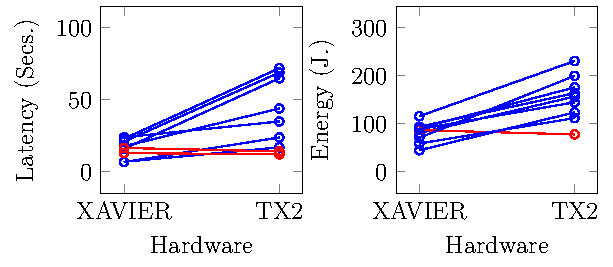
\includegraphics[width=\linewidth]{figures-vg/lineplot_multienv.pdf}
%     \caption{Ranking of configurations may change across environments, here between two hardware (\xavier and \txtwo). The reason can be associated with differences in microarchitecture and different hardware resources.}
%     \label{fig:multi_env_change}
% \end{figure}

% Causal performance models capture the underlying causal mechanisms and use them for performance-related tasks in the new environments. On the other hand, performance influence models need to relearn the patterns from scratch, therefore, they demand more samples in the new environments.
\begin{table}[]
\centering
\caption{Hyperparameters for FCI used in \ourapproach.}
\begin{tabular}{lll}
\hline
Hyperparameters & Value \\
\hline 
\texttt{depth} &-1 \\
\texttt{testId} &fisher-z-test\\
\texttt{maxPathLength} &-1 \\
\texttt{completeRuleSetUsed}&False\\
\hline 

\end{tabular}
\end{table}
% % \begin{table*}[h]
% \caption{\small Configurations options by each layer.}
% \small 
% \resizebox{\linewidth}{!}{\begin{tabular}[t]{p{0.35\linewidth}|p{0.3\linewidth}p{0.2\linewidth}p{0.2\linewidth}p{0.2\linewidth}}
 
% \centering
% Configuration options& & Layer&\\
% \midrule
% \multicolumn{5}{c}{Workload}\\
% \cmidrule(lr){1-5}\\ 
% &\multicolumn{4}{c}{DNN}\\
% \cmidrule(lr){2-5}\\
% Memory growth & 0, 0.1, 0.5&\\
% Logical devices & 10, 50\\ 
% \cmidrule(lr){2-5}\\
% &\multicolumn{4}{c}{SQLite}\\
% \cmidrule(lr){2-5}\\
% Cache size & 0, 0.1, 0.5&\\
% Buffer size & 10, 50\\ 
% Synchronous & 0, 1 \\
% Journal mode & Memory, Disk \\
% Temporary store & Memory, Disk \\

% \cmidrule(lr){2-5}\\
% &\multicolumn{4}{c}{x264}\\
% \cmidrule(lr){2-5}\\
% CRF & 0, 0.1, 0.5&\\
% Preset & 10, 50\\
% Bit rate & 10,100\\
% Latency & 1,2 \\
% \hline 
% \multicolumn{5}{c}{OS/Kernel}\\
% \cmidrule{1-5}\\
% Scheduler policy& CFP, NOOP\\
% Swappiness&10, 60, 100\\
% Dirty background ratio&10, 80\\
% Dirty ratio& 5, 50\\
% Sched child runs first & 0, 1 \\
% Drop caches & 0, 1, 2, 3\\
% Cache pressure & 1, 100, 500 \\

% \hline
% \multicolumn{5}{c}{Hardware}\\
% \cmidrule{1-5}\\
% & \multicolumn{1}{l}{\nano}&\multicolumn{1}{l}{\txone} & \multicolumn{1}{l}{\txtwo} & \multicolumn{1}{l}{\xavier}\\
% \cmidrule{2-2}\cmidrule{3-3}\cmidrule{4-4}\cmidrule{5-5}\\
% Active CPUs&1 - 4&1 - 4&1 - 4&1 - 4\\
% CPU freq. (GHz)&0.3 - 2.0&0.3 - 2.0&0.3 - 2.0&0.3 - 2.0\\
% GPU freq. (GHz)& 0.1 - 1.3&0.3 - 2.0&0.3 - 2.0&0.3 - 2.0\\
% EMC freq. (GHz)&0.1 - 1.8&0.3 - 2.0&0.3 - 2.0&0.3 - 2.0\\

% \bottomrule
% \end{tabular}}
% \label{tab:configurations}
% \end{table*}%}




\subsubsection{Case Study.}
~\fig{real_wrold_cpm} shows the causal graph to resolve the real-world latency fault.

\begin{figure}[t!]
\small
    % \setlength{\belowcaptionskip}{-3em}
    \centering
    \includegraphics*[width=\linewidth]{figures-vg/fig__realworld.pdf}
    \caption{\small {Causal graph used to resolve the latency fault in the real world case study in section~\ref{sec:casestudy}}}
    \label{fig:real_wrold_cpm}
    
\end{figure}

\begin{table*}[h]
    \centering
    \caption{\small  Efficiency of \ourapproach compared to other approaches. Cells highlighted in \colorbox{blue!10}{\bfseries blue} indicate improvement over faults and \colorbox[HTML]{FFCCC9}{red} indicate deterioration. \ourapproach achieves better performance overall and is much faster.
    }
\vspace{-0.85em}
\subfloat[Single objective performance fault for \textit{heat} in \txone.]{\scriptsize
    \label{tab:rq1_1}
    \resizebox{\textwidth}{!}{
    \begin{tabular}{@{}l|l|l|lllll|lllll|lllll|lllll|ll|}
        \clineB{4-25}{2}
        \multicolumn{1}{c}{}&\multicolumn{1}{c}{}  &  & \multicolumn{5}{c|}{Accuracy} & \multicolumn{5}{c|}{Precision} & \multicolumn{5}{c|}{Recall} & \multicolumn{5}{c|}{Gain} & \multicolumn{2}{c|}{Time$^\dagger$} \bigstrut\\ \clineB{4-25}{2}
        \multicolumn{1}{c}{}& \multicolumn{1}{c}{} &  & \multicolumn{1}{c}{\rotatebox{90}{\bfseries \ourapproach}} &
        \multicolumn{1}{c}{\rotatebox{90}{\cbi}} & \multicolumn{1}{c}{\rotatebox{90}{DD}} & \multicolumn{1}{c}{\rotatebox{90}{\encore}} & \multicolumn{1}{c|}{\rotatebox{90}{\bugdoc~}} & \multicolumn{1}{c}{\rotatebox{90}{\bfseries \ourapproach}} &  
        \multicolumn{1}{c}{\rotatebox{90}{\cbi}} & \multicolumn{1}{c}{\rotatebox{90}{DD}} & \multicolumn{1}{c}{\rotatebox{90}{\encore}} & \multicolumn{1}{c|}{\rotatebox{90}{\bugdoc~}} & \multicolumn{1}{c}{\rotatebox{90}{\bfseries \ourapproach}} &
        \multicolumn{1}{c}{\rotatebox{90}{\cbi}} & \multicolumn{1}{c}{\rotatebox{90}{DD}} & \multicolumn{1}{c}{\rotatebox{90}{\encore}} & \multicolumn{1}{c|}{\rotatebox{90}{\bugdoc~}} & \multicolumn{1}{c}{\rotatebox{90}{\bfseries \ourapproach}} & \multicolumn{1}{c}{\rotatebox{90}{\cbi}} & \multicolumn{1}{c}{\rotatebox{90}{DD}} & \multicolumn{1}{c}{\rotatebox{90}{\encore}} & \multicolumn{1}{c|}{\rotatebox{90}{\bugdoc
        ~}} & \multicolumn{1}{c}{\rotatebox{90}{\bfseries \ourapproach}} &  \multicolumn{1}{c|}{\rotatebox{90}{Others}} \bigstrut[t]
        \\ \clineB{4-25}{2}
    \multicolumn{1}{c}{}&\multicolumn{1}{c}{}  & \multicolumn{1}{c}{} & \multicolumn{1}{c}{} & \multicolumn{1}{c}{} & \multicolumn{1}{c}{} & \multicolumn{1}{c}{} & \multicolumn{1}{c}{} \bigstrut\\[-1.4em]\hlineB{2}
    
     &  & \textsc{Xception} & \cellcolor{blue!10}\bfseries69 & 63 & 57 & 64 & 65 & \cellcolor{blue!10}\bfseries 75 & 56 & 56 & 60 & 66 & \cellcolor{blue!10}\bfseries68  & 62 & 58 & 64 & 69 & \cellcolor{blue!10}\bfseries4  & 3 & 2 & 2 & 3 & \cellcolor{blue!10}\bfseries0.6 &4 \\
     
     &  & \textsc{BERT} & \cellcolor{blue!10}\bfseries71 &62 & 61 & 61 & 62 & \cellcolor{blue!10}\bfseries72  & 56 & 59 & 56 & 61 & \cellcolor{blue!10}\bfseries 72 & 65 & 62 & 67 & 62 & \cellcolor{blue!10}\bfseries5  & 3 & 2 & 2 & 3 & \cellcolor{blue!10}\bfseries0.4 & 4 \\
     
     &  & \textsc{Deepspeech} & \cellcolor{blue!10}\bfseries71  & 61 & 64 & 62 & 67 & \cellcolor{blue!10}\bfseries71  & 58 & 59 & 54 & 68 & \cellcolor{blue!10}\bfseries69  & 67 & 66 & 68 & 67 & \cellcolor{blue!10}\bfseries3 & 3 & 2 & 2 & 2 & \cellcolor{blue!10}\bfseries0.7  & 4 \\
     
     & \multirow{-4}{*}{\rotatebox{90}{Heat}} & \textsc{x264} & \cellcolor{blue!10}\bfseries74  & 65 & 57 & 64 & 65 & \cellcolor{blue!10}\bfseries74  &62 & 54 & 55 & 65 & \cellcolor{blue!10}\bfseries74 & 66 & 63 & 68 & 69 & \cellcolor{blue!10}\bfseries7  & 3 & 2 & 2 & 5 & \cellcolor{blue!10}\bfseries1.4  & 4 \\ \hlineB{2}
    \end{tabular}
    }}
    \\
    \subfloat[Multi-objective non-functional faults for \textit{Heat, Latency} in \txtwo.]{
        \scriptsize
        \label{tab:rq2}
        \resizebox{\textwidth}{!}{
            \begin{tabular}{@{}r@{}ll|llll|llll|llll|llll|llll|ll|}
            \clineB{4-25}{2}
            &  &  & \multicolumn{4}{c|}{Accuracy} & \multicolumn{4}{c|}{Precision} & \multicolumn{4}{c|}{Recall} & \multicolumn{4}{c|}{Gain (Latency)} & \multicolumn{4}{c|}{Gain (Heat)}  & \multicolumn{2}{c|}{Time$^\dagger$} \bigstrut\\ \clineB{4-25}{2}
            % &  &  &  &  &  &  &  &  & \\[-1em]\clineB{4-29}{2} 
            
            &  &  & \rotatebox{90}{\bfseries \ourapproach~} & \rotatebox{90}{\cbi} & \rotatebox{90}{\encore} & \rotatebox{90}{\bugdoc} & \rotatebox{90}{\bfseries \ourapproach~}  & \rotatebox{90}{\cbi} & \rotatebox{90}{\encore} & \rotatebox{90}{\bugdoc} & \rotatebox{90}{\bfseries \ourapproach~} & \rotatebox{90}{\cbi} & \rotatebox{90}{\encore} & \rotatebox{90}{\bugdoc} & \rotatebox{90}{\bfseries \ourapproach~} & \rotatebox{90}{\cbi} & \rotatebox{90}{\encore} & \rotatebox{90}{\bugdoc} & \rotatebox{90}{\bfseries \ourapproach~} & \rotatebox{90}{\cbi} & \rotatebox{90}{\encore} & \rotatebox{90}{\bugdoc} & \rotatebox{90}{\bfseries \ourapproach~}  & \rotatebox{90}{Others} \\ \clineB{4-25}{2}
            
            \multicolumn{1}{l}{}&\multicolumn{1}{l}{}  & \multicolumn{1}{l}{} & \multicolumn{1}{l}{} & \multicolumn{1}{l}{} & \multicolumn{1}{l}{} & \multicolumn{1}{l}{} & \multicolumn{1}{l}{} & \multicolumn{1}{l}{} & \multicolumn{1}{l}{} \\[-0.85em]\hlineB{2}

            & \multicolumn{1}{l|}{} & \textsc{Xception} & \cellcolor{blue!10}\textbf{62} & 52 & 55 & 57 & \cellcolor{blue!10}\textbf{69} & 57 & 50 & 61 & \cellcolor{blue!10}\textbf{61} & 48 &51 & 60 & \cellcolor{blue!10}\textbf{58} & 42 & 47 & 51 & \cellcolor{blue!10}\textbf{2} & 1 & 1 & 1 & \cellcolor{blue!10}\textbf{0.9} & 4 \\
            
            & \multicolumn{1}{l|}{} & \textsc{BERT} & \cellcolor{blue!10}\textbf{64} & 52 & 47 & 56 & \cellcolor{blue!10}\textbf{62} & 52 & 45 & 60 & \cellcolor{blue!10}\textbf{68} & 54  & 62 & 65 & \cellcolor{blue!10}\textbf{65} & 37 & 48 & 60 & \cellcolor{blue!10}\textbf{4}  & 3 & 2 & 3 & \cellcolor{blue!10}\textbf{0.4}  & 4 \\
            
            & \multicolumn{1}{l|}{} & \textsc{Deepspeech} & \cellcolor{blue!10}\textbf{62}  & 52 & 43 & 55 & \cellcolor{blue!10}\textbf{60} & 48 & 48 & 55 & \cellcolor{blue!10}\textbf{67}  & 58 & 41 & 59 & \cellcolor{blue!10}\textbf{69}  & 37 & 45 & 65 & \cellcolor{blue!10}\textbf{4}  & 1 & 1 & 4  & \cellcolor{blue!10}\textbf{0.3}  & 4 \\
            
            \multirow{-4}{*}{\rotatebox{90}{Latency +}} & \multicolumn{1}{l|}{\multirow{-4}{*}{\rotatebox{90}{Heat}}} & \multicolumn{1}{l|}{\textsc{x264}} & \cellcolor{blue!10}\textbf{61}  & 53 & 53 & 60 & \cellcolor{blue!10}\textbf{63}  & 50 & 54 & 61 & \cellcolor{blue!10}\textbf{60}  & 53 & 55 & 55 & \cellcolor{blue!10}\textbf{67}  & 54 & 54 & 65 & \cellcolor{blue!10}\textbf{5}  & 3 & 3 & 4  & \cellcolor{blue!10}\textbf{0.5}  & 4 \\
            \multicolumn{1}{l}{}&\multicolumn{1}{l}{}  & \multicolumn{1}{l}{} & \multicolumn{1}{l}{} & \multicolumn{1}{l}{} & \multicolumn{1}{l}{} & \multicolumn{1}{l}{} & \multicolumn{1}{l}{} & \multicolumn{1}{l}{} & \multicolumn{1}{l}{} \\[-0.85em]\hlineB{2}
          
           
           \end{tabular}
           
    }}
     \\
    \subfloat[Multi-objective non-functional faults for \textit{Energy, Heat} in \xavier.]{
        \scriptsize
        \label{tab:rq2}
        \resizebox{\textwidth}{!}{
            \begin{tabular}{@{}r@{}ll|llll|llll|llll|llll|llll|ll|}
            \clineB{4-25}{2}
            &  &  & \multicolumn{4}{c|}{Accuracy} & \multicolumn{4}{c|}{Precision} & \multicolumn{4}{c|}{Recall} & \multicolumn{4}{c|}{Gain (Energy)} & \multicolumn{4}{c|}{Gain (Heat)}  & \multicolumn{2}{c|}{Time$^\dagger$} \bigstrut\\ \clineB{4-25}{2}
            % &  &  &  &  &  &  &  &  & \\[-1em]\clineB{4-29}{2} 
            
            &  &  & \rotatebox{90}{\bfseries \ourapproach~} & \rotatebox{90}{\cbi} & \rotatebox{90}{\encore} & \rotatebox{90}{\bugdoc} & \rotatebox{90}{\bfseries \ourapproach~}  & \rotatebox{90}{\cbi} & \rotatebox{90}{\encore} & \rotatebox{90}{\bugdoc} & \rotatebox{90}{\bfseries \ourapproach~} & \rotatebox{90}{\cbi} & \rotatebox{90}{\encore} & \rotatebox{90}{\bugdoc} & \rotatebox{90}{\bfseries \ourapproach~} & \rotatebox{90}{\cbi} & \rotatebox{90}{\encore} & \rotatebox{90}{\bugdoc} & \rotatebox{90}{\bfseries \ourapproach~} & \rotatebox{90}{\cbi} & \rotatebox{90}{\encore} & \rotatebox{90}{\bugdoc} & \rotatebox{90}{\bfseries \ourapproach~}  & \rotatebox{90}{Others} \\ \clineB{4-25}{2}
            
            \multicolumn{1}{l}{}&\multicolumn{1}{l}{}  & \multicolumn{1}{l}{} & \multicolumn{1}{l}{} & \multicolumn{1}{l}{} & \multicolumn{1}{l}{} & \multicolumn{1}{l}{} & \multicolumn{1}{l}{} & \multicolumn{1}{l}{} & \multicolumn{1}{l}{} \\[-0.85em]\hlineB{2}

            & \multicolumn{1}{l|}{} & \textsc{Xception} & \cellcolor{blue!10}\textbf{65} & 55 & 57 & 63 & \cellcolor{blue!10}\textbf{64} & 55 & 51 & 62 & \cellcolor{blue!10}\textbf{67} & 47 &53 & 60 & \cellcolor{blue!10}\textbf{58} & 44 & 51 & 54 & \cellcolor{blue!10}\textbf{3} & 1 & 1 & 1 & \cellcolor{blue!10}\textbf{0.8} & 4 \\
            
            & \multicolumn{1}{l|}{} & \textsc{BERT} & \cellcolor{blue!10}\textbf{69} & 55 & 51 & 59 & \cellcolor{blue!10}\textbf{65} & 53 & 47 & 61 & \cellcolor{blue!10}\textbf{71} & 53 & 61 & 67 & \cellcolor{blue!10}\textbf{65} & 41 & 51& 61 & \cellcolor{blue!10}\textbf{4}  & 2 & 2 & 3 & \cellcolor{blue!10}\textbf{0.4}  & 4 \\
            
            & \multicolumn{1}{l|}{} & \textsc{Deepspeech} & \cellcolor{blue!10}\textbf{72}  & 55 & 49 & 61 & \cellcolor{blue!10}\textbf{73} & 51 & 51 & 61 & \cellcolor{blue!10}\textbf{71}  & 57 & 53 & 64 & \cellcolor{blue!10}\textbf{69}  & 47 & 51 & 64 & \cellcolor{blue!10}\textbf{4}  & 1 & 1 & 3  & \cellcolor{blue!10}\textbf{0.3}  & 4 \\
            
            \multirow{-4}{*}{\rotatebox{90}{Energy +}} & \multicolumn{1}{l|}{\multirow{-4}{*}{\rotatebox{90}{Heat}}} & \multicolumn{1}{l|}{\textsc{x264}} & \cellcolor{blue!10}\textbf{72}  & 59 & 57 & 66 & \cellcolor{blue!10}\textbf{71}  & 51 & 55 & 62 & \cellcolor{blue!10}\textbf{69}  & 61 & 59 & 59 & \cellcolor{blue!10}\textbf{67}  & 51 & 51 & 61 & \cellcolor{blue!10}\textbf{5}  & 2 & 3 & 4  & \cellcolor{blue!10}\textbf{0.5}  & 4 \\
            \multicolumn{1}{l}{}&\multicolumn{1}{l}{}  & \multicolumn{1}{l}{} & \multicolumn{1}{l}{} & \multicolumn{1}{l}{} & \multicolumn{1}{l}{} & \multicolumn{1}{l}{} & \multicolumn{1}{l}{} & \multicolumn{1}{l}{} & \multicolumn{1}{l}{} \\[-0.85em]\hlineB{2}
          
           
           \end{tabular}
           
    }}
    \\
    \subfloat[Multi-objective non-functional faults for \textit{Energy, Heat, and Latency} in \txtwo.]{
        \scriptsize
          

    \footnotesize
    \resizebox{\linewidth}{!}{
        \begin{tabular}{@{}l@{}ll|llll|llll|llll|llll|llll|llll|ll|}
            \clineB{4-29}{2}
            &  &  & \multicolumn{4}{c|}{Accuracy} & \multicolumn{4}{c|}{Precision} & \multicolumn{4}{c|}{Recall} & \multicolumn{4}{c|}{Gain (Latency)} & \multicolumn{4}{c|}{Gain (Energy)} & \multicolumn{4}{c|}{Gain (Heat)} & \multicolumn{2}{c|}{Time$^\dagger$} \bigstrut\\ \clineB{4-29}{2}
            % &  &  &  &  &  &  &  &  & \\[-1em]\clineB{4-29}{2} 
            
            &  &  & \rotatebox{90}{\bfseries\ourapproach~} & \rotatebox{90}{\cbi} & \rotatebox{90}{\encore} & \rotatebox{90}{\bugdoc} & \rotatebox{90}{\bfseries\ourapproach~} & \rotatebox{90}{\cbi} & \rotatebox{90}{\encore} & \rotatebox{90}{\bugdoc} & \rotatebox{90}{\bfseries\ourapproach~} & \rotatebox{90}{\cbi} & \rotatebox{90}{\encore} & \rotatebox{90}{\bugdoc} & \rotatebox{90}{\bfseries\ourapproach~} & \rotatebox{90}{\cbi} & \rotatebox{90}{\encore} & \rotatebox{90}{\bugdoc} & \rotatebox{90}{\bfseries\ourapproach~} & \rotatebox{90}{\cbi} & \rotatebox{90}{\encore} & \rotatebox{90}{\bugdoc} & \rotatebox{90}{\bfseries\ourapproach~} & \rotatebox{90}{\cbi} & \rotatebox{90}{\encore} & \rotatebox{90}{\bugdoc} & \rotatebox{90}{\bfseries\ourapproach~} & \rotatebox{90}{Others} \\ \clineB{4-29}{2}
            
           \multicolumn{1}{l}{}&\multicolumn{1}{l}{}  & \multicolumn{1}{l}{} & \multicolumn{1}{l}{} & \multicolumn{1}{l}{} & \multicolumn{1}{l}{} & \multicolumn{1}{l}{} & \multicolumn{1}{l}{} & \multicolumn{1}{l}{} & \multicolumn{1}{l}{} \\[-0.95em]\hlineB{2}

            & \multicolumn{1}{l|}{} & Image & \cellcolor{blue!10}\textbf{76} & 57 & 48 & 66 & \cellcolor{blue!10}\textbf{68} & 61 & 57 & 61 & \cellcolor{blue!10}\textbf{81} & 53 & 46 & 70 & \cellcolor{blue!10}\textbf{62} & 33 & 30 & 42 & \cellcolor{blue!10}\textbf{52} & 23 & 18 & 24 & \cellcolor{blue!10}\textbf{4} & 1 & 0 & 0 & \cellcolor{blue!10}\textbf{0.1} & 4 \\
            & \multicolumn{1}{l|}{} & x264 & \cellcolor{blue!10}\textbf{80} & 59 & 47 & 54 & \cellcolor{blue!10}\textbf{76} & 61 & 56 & 63 & \cellcolor{blue!10}\textbf{81} & 56 & 46 & 51 & \cellcolor{blue!10}\textbf{12} & 2 & 1 & 2 & \cellcolor{blue!10}\textbf{15} & 4 & 2 & 4 & \cellcolor{blue!10}\textbf{4} & 1 & 0 & 1 & \cellcolor{blue!10}\textbf{0.1} & 4 \\
           \multirow{-3}{*}{\rotatebox{90}{All}} & \multicolumn{1}{l|}{\multirow{-3}{*}{\rotatebox{90}{Three}}} & SQLite & \cellcolor{blue!10}\textbf{73} & 56 & 51 & 53 & \cellcolor{blue!10}\textbf{68} & 59 & 56 & 60 & \cellcolor{blue!10}\textbf{78} & 54 & 45 & 51 & \cellcolor{blue!10}\textbf{12} & 1 & 1 & 4 & \cellcolor{blue!10}\textbf{8} & 4 & 2 & 5 & \cellcolor{blue!10}\textbf{1} & 1 & \cellcolor[HTML]{FFCCC9}-1 & \cellcolor[HTML]{FFCCC9}-1 & \cellcolor{blue!10}\textbf{0.1} & 4 \\ \hlineB{2}
           \multicolumn{10}{l}{$^\dagger$ Wallclock time in hours}\bigstrut
           \end{tabular}
    }}
    \label{tab:rq_effectiveness_appendix}
\end{table*}


% To understand how \tool scales in such scenarios, we evaluate \tool by increasing the number of values the software, hardware, and kernel configuration options can be set to while resolving the latency faults in the SQLite. %There are two scenarios in this case: (a) 242 configurations and 88 system events when we select all the modifiable software/hardware configurations and events and (b) 242 configurations and 288 events when we select not only all modifiable software and hardware configurations and system events but also intermediate {\tt tracepoint events}. 
% In the second case, we increase the granularity of kernel configurations by considering all the permitted values by \texttt{Linux} kernel. As system events can only be observed, we increase the granularity of events by observing the tracepoint events along with hardware/software events. 
% % Similar to {RQ3-A.}, we track the time required to discover the causal structure, evaluate the counterfactual queries, and total time to resolve latency faults.

\subsubsection{Effectiveness.}
~\Cref{tab:rq_effectiveness_appendix}(a) shows the effectiveness of \ourapproach in resolving single objective faults due to heat in NVIDIA \txone. Here, \ourapproach ~{ outperforms correlation-based methods in all cases}. For example, in  \textsc{Bert} on TX1, \ourapproach achieves 9\% more accuracy, 11\% more precision, and 10\% more recall compared to the next best method, \bugdoc. We observed heat gains as high as $7\%$ ($2\%$ more than \bugdoc) on \textsc{x264}. The results confirm that \ourapproach~{\em can recommend repairs for faults that significantly improve latency and energy usage}. Applying the changes to the configurations recommended by \ourapproach increases the performance drastically. 



\ourapproach~{\em can resolve misconfiguration faults significantly faster than correlation-based approaches}.~In~\Cref{tab:rq_effectiveness_appendix}, the last two columns indicate the time taken (in hours) by each approach to diagnosing the root cause. \ourapproach can do resolve faults significantly faster, \eg, \ourapproach is $13\times$ faster in diagnosing and resolving latency and heat faults for \textsc{Deepspeech}. 




\subsubsection{Transferability.}
\begin{table}
    \caption{\small Transferring causal models across hardware platforms. Cells highlighted in \colorbox{blue!10}{\bfseries blue} indicate the transferability potential of \ourapproach when compared to \ourapproach \textsc(Rerun).  }
    \label{tab:transfer}
    \centering
    \resizebox{\linewidth}{!}{
    \begin{tabular}{ll|rrr|rrr|rrr|rrr}
        \hlineB{2}
        \multicolumn{14}{c}{TX1 (source) $\longrightarrow$ TX2 (target)} \bigstrut\\ \hlineB{2}

        & \multicolumn{1}{l|}{} & \multicolumn{3}{c|}{Accuracy} & \multicolumn{3}{c|}{Recall} & \multicolumn{3}{c|}{Precision} & \multicolumn{3}{c}{$\Delta_{gain}$} 
        
        \bigstrut\\ \clineB{3-14}{2} 
        
        &  Software & \rotatebox{90}{\ourapproach \textsc{(Reuse)}} & \multicolumn{1}{r}{\rotatebox{90}{\ourapproach+25}} & \rotatebox{90}{\ourapproach \textsc{(Rerun)}} & \rotatebox{90}{\ourapproach \textsc{(Reuse)}} & \multicolumn{1}{r}{\rotatebox{90}{\ourapproach+25}} & \rotatebox{90}{\ourapproach \textsc{(Rerun)}} & \rotatebox{90}{\ourapproach \textsc{(Reuse)}} & \multicolumn{1}{r}{\rotatebox{90}{\ourapproach+25}} & \rotatebox{90}{\ourapproach \textsc{(Rerun)}} & \rotatebox{90}{\ourapproach \textsc{(Reuse)}} & \multicolumn{1}{r}{\rotatebox{90}{\ourapproach+25}} & \rotatebox{90}{\ourapproach \textsc{(Rerun)}} \bigstrut\\ \hlineB{2}       

    \multicolumn{1}{l|}{\multirow{5}{*}{\rotatebox{90}{Latency}}} & \textsc{Xception} & 52 & \cellcolor{blue!10}83 & 86 & 70 & \cellcolor{blue!10}79 & 86 & 46 & \cellcolor{blue!10}78 & 83 & 46 & \cellcolor{blue!10}71 & 82 \bigstrut\\
    \multicolumn{1}{l|}{} & \textsc{Bert} & 55 & \cellcolor{blue!10}75 & 81 & 57 & \cellcolor{blue!10}70 & 71 & 45 & \cellcolor{blue!10}67 & 76 & 43 & \cellcolor{blue!10}70 & 74 \bigstrut\\
    \multicolumn{1}{l|}{} & \textsc{Deepspeech} & 45 & \cellcolor{blue!10}71 & 81 & 56 & \cellcolor{blue!10}79 & 81 & 49 & \cellcolor{blue!10}73 & 76 & 54 & \cellcolor{blue!10}73 & 76 \bigstrut\\
    \multicolumn{1}{l|}{} & \textsc{x264} & 57 & \cellcolor{blue!10}79 & 83 & 70 & \cellcolor{blue!10}75 & 78 & 58 & \cellcolor{blue!10}77 & 82 & 45 & \cellcolor{blue!10}73 & 85 \bigstrut\\
     \hlineB{2}
    \multicolumn{14}{c}{TX2 (source) $\longrightarrow$ \xavier (target)} \bigstrut\\ \hlineB{2}
    \multicolumn{1}{l|}{\multirow{5}{*}{\rotatebox{90}{Energy}}} & \textsc{Xception} & 53 & \cellcolor{blue!10}74 & 84 & 48 & \cellcolor{blue!10}73 & 80 & 51 & \cellcolor{blue!10}69 & 78 & 43 & \cellcolor{blue!10}73 & 83 \bigstrut\\
    \multicolumn{1}{l|}{} & \textsc{Bert} & 50 & \cellcolor{blue!10}61 & 66 & 53 & \cellcolor{blue!10}71 & 79 & 49 & \cellcolor{blue!10}66 & 70 & 40 & \cellcolor{blue!10}55 & 62 \bigstrut\\
    \multicolumn{1}{l|}{} & \textsc{Deepspeech} & 57 & \cellcolor{blue!10}70 & 73 & 45 & \cellcolor{blue!10}74 & 78 & 43 & \cellcolor{blue!10}69 & 75 & 49 & \cellcolor{blue!10}71 & 78 \bigstrut\\
    \multicolumn{1}{l|}{} & \textsc{x264} & 54 & \cellcolor{blue!10}72 & 77 & 46 & \cellcolor{blue!10}72 & 78 & 42 & \cellcolor{blue!10}75 & 83 & 46 & \cellcolor{blue!10}79 & 87 \bigstrut\\
    \hlineB{2}
    \multicolumn{14}{c}{\xavier (source) $\longrightarrow$ TX1 (target)} \bigstrut\\ \hlineB{2}
    \multicolumn{1}{l|}{\multirow{5}{*}{\rotatebox{90}{Heat}}} & \textsc{Xception}& 63 & \cellcolor{blue!10}64 & 69 & 61 & \cellcolor{blue!10}67 & 68 & 58 & \cellcolor{blue!10}74 & 75 & 3 & \cellcolor{blue!10}4 & 4 \bigstrut\\
    \multicolumn{1}{l|}{} & \textsc{Bert} & 55 & \cellcolor{blue!10}65 & 71 & 59 & \cellcolor{blue!10}67 & 72 & 52 & \cellcolor{blue!10}64 & 72 & 3 & \cellcolor{blue!10}4 & 5 \bigstrut\\
    \multicolumn{1}{l|}{} & \textsc{Deepspeech} & 57 & \cellcolor{blue!10}64 & 71 & 59 & \cellcolor{blue!10}63 & 69 & 53 & \cellcolor{blue!10}63 & 71 & 1 & \cellcolor{blue!10}2 & 3 \bigstrut\\
    \multicolumn{1}{l|}{} & \textsc{x264} & 51 & \cellcolor{blue!10}65 & 74 & 53 & \cellcolor{blue!10}64 & 74 & 54 & \cellcolor{blue!10}69 & 74 & 3 & \cellcolor{blue!10}5 & 7 \bigstrut\\
     \hlineB{2}
    \end{tabular}}
    \end{table}
    
Table~\ref{tab:transfer} indicates the results for different transfer scenarios: (I) We learn a causal model from \txone and use them to resolve the latency faults in \txtwo,  (I) We learn a causal model from \txtwo and use them to resolve the energy faults in \xavier, and (III) We learn a causal model from \xavier and use them to resolve the heat faults in \txone. Here, we determine how transferable is \ourapproach by comparing with \ourapproach \textsc(Reuse), \ourapproach+25, and \ourapproach \textsc(Rerun). For all systems, we observe that the performance of \ourapproach \textsc(Reuse) is close to the performance of \ourapproach \textsc(Rerun) which confirms the high transferability property of \ourapproach. For example, in \textsc{Xception} and \textsc{SQLite}, \ourapproach \textsc(Reuse) has the exact gain as of \ourapproach \textsc(Rerun) for heat faults. For latency and energy faults, the main difference between \ourapproach \textsc(Reuse) and \ourapproach \textsc(Rerun) is less than 5\% for all systems. We also observe that with little updates, \ourapproach+25 ($\sim$24 minutes) achieves a similar performance of \ourapproach \textsc{(Rerun)} ($\sim$40 minutes), on average. This confirms that as the causal mechanisms are sparse, the causal performance model from source in \ourapproach quickly reaches a fixed structure in the target using incremental learning by judiciously evaluating the most promising fixes until the fault is resolved.

\subsubsection{Scalability.}

The scalability of \ourapproach depends on the scalability of each phase. Therefore, we design scenarios to test the scalability of each phase to determine the overall scalability. Since the initial number of samples and the underlying phases for each task is the same, it is sufficient to examine the scalability of \ourapproach for the debugging non-functional fault task. 

 
\textsc{SQLite} was chosen because it offers a large number of configurable options, much more than neural applications, and video encoders. Further, each of these options can take on a large number of permitted values, making \textsc{Deepstream} a useful candidate to study the scalability of \ourapproach. \textsc{Deepstream} was chosen as it has a higher number of components than others, and it is interesting to determine how \ourapproach behaves when the number of options and events are increasing. As a result, SQLite exposes new system design opportunities to enable efficient inference and many complex interactions between software options. 


In large systems, there are significantly more causal paths and therefore, causal learning and estimations of queries take more time. However, with as many as 242 configuration options and 19 events (\tab{scalability}, row 2), causal graph discovery takes roughly one minute, evaluating all 2234 queries takes roughly two minutes, and the total time to diagnose and fix a fault is roughly 22 minutes for \textsc{SQLite}. This trend is observed even with 242 configuration options, 288 events (\tab{scalability}, row 3), and finer granularity of configuration values---the time required to causal model recovery is a little over 1 minute and the total time to diagnose and fix a fault is less than 2 hours. Similarly, in \textsc{Deepstream}, with 53 configuration options and 288 events, causal model discovery is less than two minutes and the time needed to diagnose and fix a fault is less than an hour. 
The results in ~\tab{scalability} indicate that \ourapproach can scale to a much larger configuration space without an exponential increase in runtime for any of the intermediate stages. This can be attributed to the sparsity of the causal graph (average degree of a node for \textsc{SQLite} in \tab{scalability} is at most 3.6, and it reduces to 1.6 when the number of configurations increase and reduces from 3.1 to 2.3 in \textsc{Deepstream} when systems events are increased). This makes sense because not all variables (\ie, configuration options and/or system events) affect non-functional properties and a high number of variables in the graph end up as isolated nodes. Therefore, the number of paths and consequently the evaluation time do not grow exponentially as the number of variables increases.

% To understand how \ourapproach scales in such scenarios, we evaluate \ourapproach by increasing the number of values the software, hardware, and kernel configuration options can be set to while resolving the latency faults in the SQLite. From \tab{scalability} we observe that even with 242 configurations, 288 events (\tab{scalability}, row 3), and finer granularity of configuration values, the time required to causal model recovery is less than two minutes and the total time to diagnose and fix a fault is less than 2 hours. We also observe that the graph becomes more sparse (average degree of a node decreases from 1.8 to 1.6 in \tab{scalability}) and the evaluation time does not grow exponentially. 

Finally, the latency gain associated with repairs from larger configuration space with configurations was similar to the original space of 34 and 53 configurations for \textsc{SQLite} and \textsc{Deepstream}, respectively. This indicates that: (a)~imparting domain expertise to select most important configuration options can speed up the inference time of \ourapproach, and (b)~if the user chooses instead to use more configuration options (perhaps to avoid initial feature engineering), \ourapproach can still diagnose and fix faults satisfactorily within a reasonable time. 